\chapter{Introduction}
\section{Présentation du projet}
%\paragraph{Objectif}
Mettre en place, évaluer et comparer différents outils permettant de gérer de manière
centralisée et automatisée une infrastructure basée sur des machines virtuelles: Ganeti,
OpenXenManager, virt-manager, Archipel...
\section{Introduction à la virtualisation}
\subsection{Machine virtuelle}


Une machine virtuelle est un conteneur isolé capable d'exécuter
ses propres systèmes d'exploitation et application.
Une machine virtuelle se comporte exactement comme un ordinateur physique
et contient ses propres processeurs, mémoire RAM, disque dur et carte
d'interface réseau virtuel. Une machine virtuelle
a pour but de générer sur une même machine un ou plusieurs environnements
d'exécution applicative. On en distingue deux types d'applications
: d'une part la virtualisation par le biais d'un hyperviseur jouant
le rôle d'émulateur de système (PC ou serveur), d'autre part la virtualisation
applicative qui permet de faire tourner une application sur un poste
client quelque soit le système sous-jacent.

\subsection{Hyperviseur }


La machine virtuelle avec hyperviseur est utilisée pour générer au
dessus d'un système d'exploitation serveur, une couche logicielle sous
la forme d'un émulateur permettant de créer plusieurs environnements
d'exécution serveur. Cet émulateur se place comme un niveau supplémentaire qui se greffe sur le système d'origine.
\newpage
\subsection{Au commencement, la virtualisation des mainframes}

La virtualisation a été mise en œuvre pour la première fois il y
a plus de 30 ans par IBM pour partitionner logiquement des mainframes
en machines virtuelles distinctes. Ces partitions permettaient un
traitement « multitâche », à savoir l'exécution simultanée de plusieurs applications et processus. Étant donné que les mainframes consommaient beaucoup de ressources en même temps, le partitionnement constituait un moyen naturel de tirer pleinement parti de l'investissement matériel.


\subsection{Histoire de la virtualisation}

La virtualisation est un concept qui a été mis au point pour la première fois dans les années 1960 pour permettre la partition d'une vaste gamme de matériel mainframe et optimiser l'utilisation du matériel. De nos jours, les ordinateurs basés sur l'architecture x86 sont confrontés aux mêmes problèmes de rigidité et de sous-utilisation que les mainframes dans les années 1960. VMware a inventé la virtualisation pour la plate-forme x86 dans les années 1990 afin de répondre notamment aux problèmes de sous-utilisation, et a surmonté les nombreux défis émergeant au cours de ce processus. Aujourd'hui, VMware est devenu le leader mondial de la virtualisation x86 avec plus de 190 000 clients, dont la totalité des membres du classement Fortune 100.

\subsection{Enjeux de la virtualisation}

Actuellement, les entreprises rencontrent des besoins qui ne sont
pas couverts.

Au niveau de la sécurité, les entreprises souhaiteraient isoler les
services sur des serveurs différents. Pour la maintenance, il serait
utile d'améliorer des services tels que la disponibilité, la migration,la redondance,la flexibilité ou le temps de réponse. Il serait également bienvenu de tester, déléguer l'administration d'un système ...


Une des solutions pour répondre à ces besoins serait d'acquérir d'avantage de plateformes de travail.


La multiplication des serveurs pose cependant un certain nombre
de problèmes, augmenter sans cesse son parc informatique est impossible
pour plusieurs raisons : 
\begin{itemize}
\item Tout d'abord au niveau écologique celà entrainerait un surplus de déchets électronique, une consommation d'énergie directe et de l'énergie utilisée pour refroidir les salles serveur.
\item Au niveau de la surface utilisée, les salles machine seraient vite encombrées, puis apparaitra des problèmes tel que la nuisance sonore, le manque de puissance pour alimenter les salles serveur. 
\item Au niveau économique les coûts d'achat, de recyclage, de fonctionnement, de maintenance seraient trop chers. La mise en place de serveur de virtualisation est une solution pour résoudre ces problèmes.
\end{itemize}

Le but de la virtualisation est de donner un environnement système
au programme pour qu'il croit être dans un environnement
matériel. Pour cela, une machine virtuelle est utilisée. Ainsi, plusieurs
environnements d'exécution sont créés sur une seule
machine, dont chacun émule la machine hôte. L'utilisateur
pense posséder un ordinateur complet pour chaque système d'exploitation
alors que toutes les machines virtuelles sont isolées entre elles.


\newpage

\section{Présentation de Grid5000}
\begin{figure}
\begin{center}

\includegraphics{images/logo.png}
\caption{Logo de Grid5000}
\end{center}

\end{figure}
Aujourd’hui, grâce à Internet, il est possible
d’interconnecter des machines du monde entier pour
traiter et stocker des masses de données. Cette collection
hétérogène et distribuée de ressources de stockage et de
calcul a donné naissance à un nouveau concept : les
grilles informatiques.

L’idée de mutualiser les ressources
informatiques vient de plusieurs facteurs, évolution de la
recherche en parallélisme qui, après avoir étudié les
machines homogènes, s’est attaquée aux environnements
hétérogènes puis distribués ; besoins croissants des
applications qui nécessitent l’utilisation toujours plus
importante de moyens informatiques forcément répartis.

La notion de grille peut avoir plusieurs sens suivant le
contexte : grappes de grappes, environnements de type
GridRPC (appel de procédure à distance sur une grille).,
réseaux pair-à-pair, systèmes de calcul sur Internet, etc...
Il s’agit d’une manière générale de systèmes dynamiques,
hétérogènes et distribués à large échelle. De grand
nombre de problématiques de recherche sont soulevés
par l'informatique. Elles touchent plusieurs
domaines de l’informatique :algorithmique,
programmation, applications, réseaux.

L’objectif de GRID’5000 est de construire un instrument
pour réaliser des expériences en informatique dans le
domaine des systèmes distribués à grande échelle (GRID).

Cette plate-forme, ouverte depuis 2006 aux chercheurs, regroupe un certain nombre de sites
répartis sur le territoire national. Chaque site héberge une
ou plusieurs grappes de processeurs. Ces grappes sont
alors interconnectées via une infrastructure réseau dédiée
à 10 Gb/s fournie par RENATER. À ce jour, GRID’5000
est composée de 9 sites: Lille, Rennes, Orsay, Nancy,
Bordeaux, Lyon, Grenoble, Toulouse et Nice.

Début 2007, GRID’5000 regroupait plus de 2500 processeurs et près
de 3500 cœurs.

\newpage
\begin{figure}
\begin{center}
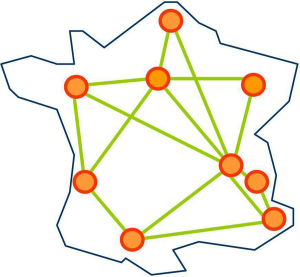
\includegraphics{images/g5k.png}
\\
\underline{\textit{Répartition des sites}}
\end{center}
\end{figure}



  \subsection{Infrastructure des sites}
Chaque site héberge :
\begin{itemize}
\item un frontend, serveur permettant d'accéder aux clusters disponibles ,
\item un serveur de données, pour centraliser les données utilisateurs ,
\item plusieurs clusters, c'est-à-dire des grappes de machines homogènes, appelées noeuds (nodes).
\end{itemize}
\begin{center}
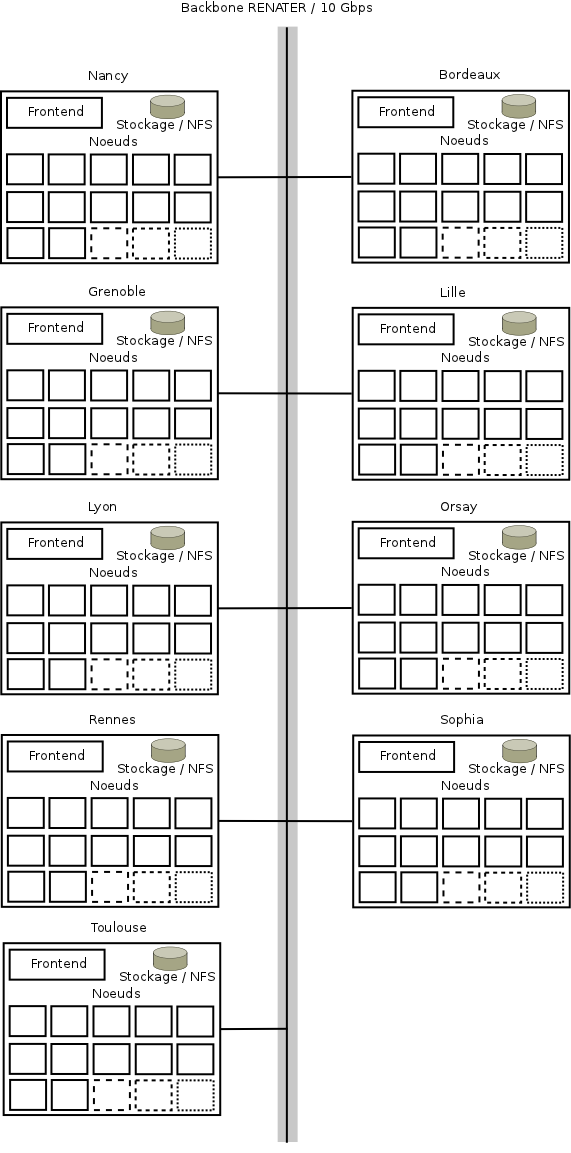
\includegraphics[width=10cm,height=15cm]{images/g5k1.png}
\\
\underline{\textit{Architecture Grid5000}}
%%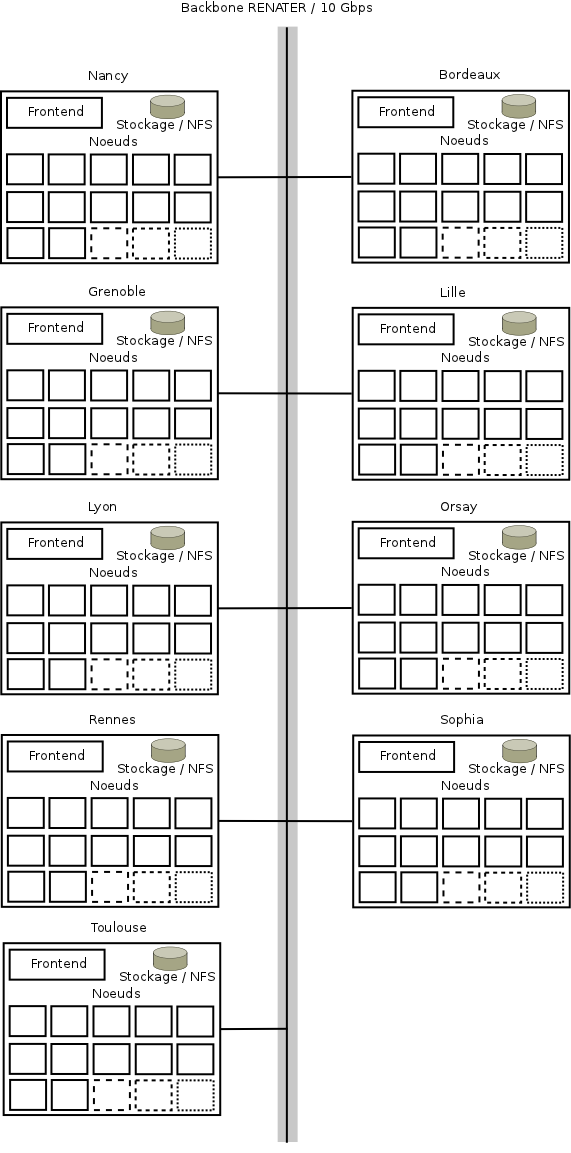
\includegraphics{images/g5k1.png}
\end{center}
L'utilisateur de Grid 5000 accède à chaque site par son frontend en utilisant le protocole SSH.\\
Commande:
\begin{lstlisting}
ssh utilisateur@access.grid5000.fr
\end{lstlisting}
Sur tous les serveurs du site, un répertoire home, local à chaque site, est monté avec NFS 2 .
A partir du frontend, il est possible d'accéder aux machines des clusters en exécutant des réservations à l'aide de la commande:
\begin{lstlisting}
oarsub
\end{lstlisting}
Grâce à notre tuteur, M. Lucas NUSSBAUM nous avons pu visiter la salle serveurs du site de Nancy située au Loria, 
et avons assisté à une présentation de la plate-forme (matériel utilisé, connexions réseau,
administration).
\newline
\emph{Une description détaillée du site de Nancy est disponible sur le site de Grid 5000.}

\subsection{Réseau}
Les sites et toutes les machines qu'ils comprennent sont interconnectés par RENATER 3 en 10Gbits/s. De
plus, chaque site peut disposer de plusieurs réseaux locaux :
\begin{itemize}
\item réseau en ethernet, 1 Gb/s
\item réseaux hautes performances (Infiniband 20 Gb/s ou 10 Gb/s, et Myrinet 20 Gb/s)
\end{itemize}

  \subsection{Environnement logiciel}
Tous les serveurs de Grid 5000 fonctionnent sous Debian GNU/Linux.
A partir du frontend, l'utilisateur peut réserver des machines en utilisant la suite de logiciels OAR dédiée à
la gestion de ressources de clusters, et déployer ses propres images de systèmes à l'aide des outils kadeploy.
Il y a deux types de réservation :
\begin{itemize}
\item par défaut, pour des besoins de calcul avec OpenMPI ;
\item pour le déploiement d'environnements (deploy ).
\end{itemize}
Dans le cadre de notre projet, nous effectuons uniquement des réservations de type deploy. La commande oarsub nous permet de réserver des nœuds sur un site (en créant un job). Voici un exemple d'utilisation d'oarsub, pour réserver 3 nœuds pendant 2 heures en déploiement.
\begin{lstlisting}
oarsub -I -t deploy -n'virtu' -l slash_22=1+nodes=3,walltime=2
\end{lstlisting}
Cette ligne nous permet de réserver 3 nœuds avec sous-réseau en /22.

Après réservation, oarsub ouvre un shell dans lequel des variables d'environnements sont définies comme \$OAR\_FILE\_NODE, qui est le nom d'un fichier avec la liste des nœuds réservés, ou \$OAR\_JOB\_ID.
\begin{lstlisting}
cat  $OAR_FILE_NODES | uniq
griffon-25. nancy . gr id5000 . f r
griffon-5. nancy . gr id5000 . f r
graphene-12. nancy . gr id5000 . f r

echo $OAR_JOB_ID
387054
\end{lstlisting}
Pour supprimer le job et libérer les ressources, on utilise la commande oardel.
\begin{lstlisting}
oardel 387054
\end{lstlisting}
Kadeploy permet de déployer des environnements personnalisés sur les noeuds réservés à l'aide d'une commande simple. Lorsque la réservation est terminée, le noeud est automatiquement restauré avec un environnement Debian ou autre.
Pour déployer un environnement sur tous les noeuds réservés, il faut utiliser la commande kadeploy3
\begin{lstlisting}
 kadeploy3 -e squeeze-x64-xen -f $OAR_FILE_NODES -k $HOME/.ssh/id_rsa.pub
\end{lstlisting}

L’option –e permet de spécifier la distribution, -f permet le déploiement sur tous les nœuds et –k permet de copier la clé ssh du frontend sur les nœuds.


\section{Répartition des tâches}
Nous avons commencé par prendre en main Grid5000 durant les 2 premières semaines du projet. Pour ce faire, nous avons suivi avec soin les tutoriels mis à notre disposition sur le site www.grid5000.fr.

Une fois les manipulations de bases bien assimilées. Nous nous sommes divisés en 2 sous-groupes pour tester les différents outils du projet :
\begin{itemize}
  \item Julien et Augustin se sont chargés de Ganeti et archipel.
  \item Sébatien et Mathieu pour OpenXenManager et virt-manager.
\end{itemize}

